\section{Organizacja pracy}

\subsection{Podział zadań w projekcie}

Realizacja projektu została podzielona między jego autorów. Do zadań poszczególnych autorów pracy należało:\\

\begin{itemize}[noitemsep,nolistsep]
\item Igor Faliszewski:
	\begin{itemize}
	\item realizacja trójwymiarowej wizualizacji symulacji,
	\item implementacja graficznego interfejsu użytkownika,
	\item obsługa interakcji z użytkownikiem,
	\item wyposażenie aplikacji w zawartość,
	\item udźwiękowienie aplikacji.
	\end{itemize}
\ \\
\item Wojciech Gajda:
	\begin{itemize}
	\item przygotowanie silnika dynamiki lotu BSP,
	\item przygotowanie silnika dynamiki obiektów niesterowalnych,
	\item przygotowanie systemu sterowania BSP,
	\item przygotowanie agregatora procesów i serwera symulacji,
	\item przygotowanie kontenera Docker z symulacją,
	\item przygotowanie generatora map.
	\end{itemize}
\end{itemize}
\ \\
Tabela (\ref{rep_rep}) prezentuje osoby odpowiedzialne za poszczególne repozytoria.

\renewcommand{\arraystretch}{1.5}
\begin{table}[!h]
\centering
\begin{tabular}{|m{0.4\textwidth}|m{0.55\textwidth}|} 
\hline
\rowcolor{Gray}
Repozytorium &  Osoba odpowiedzialna \\
\multirow{1}{15em}{Igor Faliszewski} 
& UAV\_visualization \\
\hline
\multirow{7}{15em}{{Wojciech Gajda}} 
& UAV\_aggregator \\
& UAV\_physics\_engine\\
& UAV\_controller \\
& UAV\_drop\_physic \\
& UAV\_server \\
& UAV\_map\_generator \\
& UAV\_common \\
\hline
\end{tabular}
\caption{Osoby odpowiedzialne za repozytoria}
\label{rep_rep}
\end{table}

\newpage
\subsection{Harmonogram projektu}

Prace nad projektem zostały rozpoczęte 13.03.2023. Początkowe wersje modułów były rozwijane w lokalnych repozytoriach autorów. W czerwcu 2023 rozpoczęto integrację modułu, a zagadnienia zostały opisane w programie Jira. Rysunek (\ref{zamkniete_jira}) prezentuje zagadnienia zamknięte do 15.10.2023.

\begin{figure}[!h]
\centering
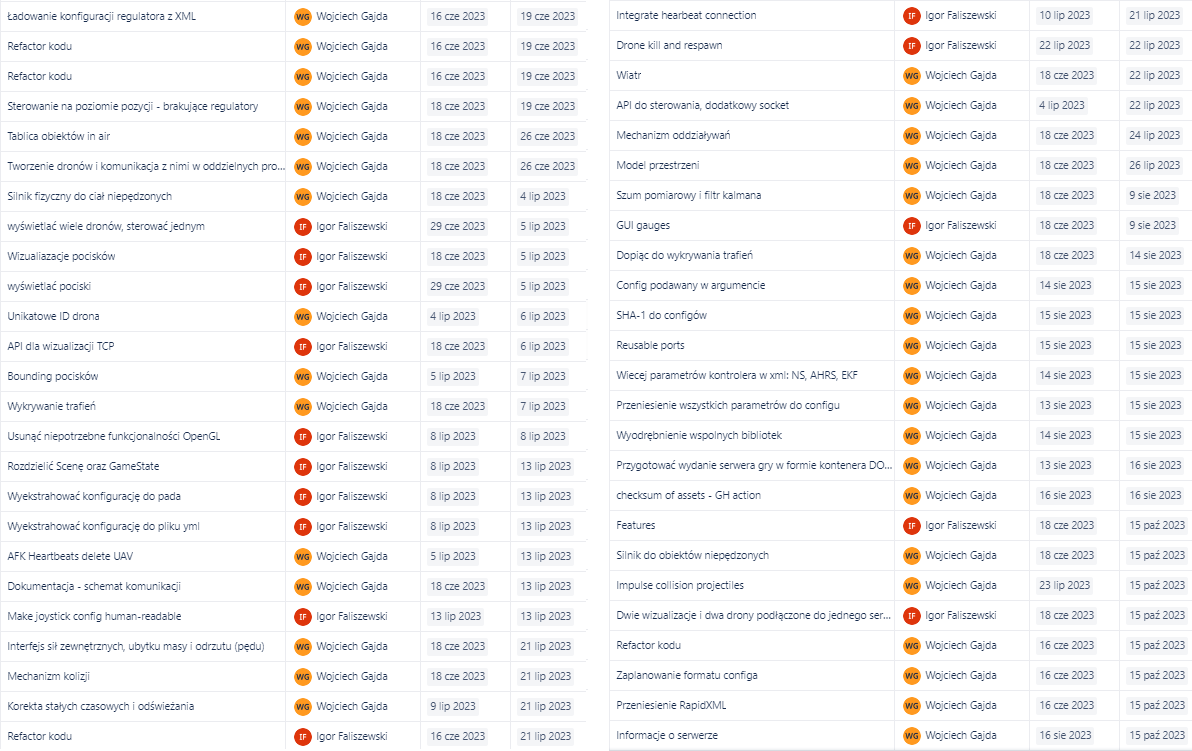
\includegraphics[width=\textwidth]{jira_june_sept.png}
\caption{Zgłoszenia zamknięte do 15.10.2023}
\label{zamkniete_jira}
\end{figure}

Na podstawie otwartych zagadnień i analizy założonej specyfikacji zaplanowany został harmonogram pracy zawierający zagadnienia, których realizacja jest niezbędna do ukończenia projektu. Tabela (\ref{harmonogram}) prezentuje ww. harmonogram. 

\renewcommand{\arraystretch}{1.5}
\begin{table}
\centering
\begin{tabular}{|m{0.4\textwidth}|m{0.15\textwidth}|m{0.15\textwidth}|m{0.2\textwidth}|} 
\hline
\rowcolor{Gray}
Opis zadania & Data\newline rozpoczęcia & Data\newline zakończenia & Osoba\newline odpowiedzialna \\
 \hline
Dodanie różnych modeli pocisków i ładunków & 16.10.2023 & 23.10.2023 & Igor Faliszewski \\
 \hline
Dodanie nowych konfiguracji rakiet & 16.10.2023 & 29.10.2023 & Wojciech Gajda \\
 \hline
Generator konfiguracji kontrolera & 24.10.2023 & 29.10.2023 & Igor Faliszewski \\ 
\hline
Implementacja nowych regulatorów płatowców & 30.10.2023 & 19.11.2023 & Wojciech Gajda \\ 
\hline
Krzywa łańcuchowa & 30.10.2023 & 12.11.2023 & Igor Faliszewski \\ 
\hline
Określanie orientacji pocisków i~ładunków & 13.11.2023 & 19.11.2023 & Igor Faliszewski \\ 
\hline
GUI wyboru pocisku i ładunku & 20.11.2023 & 26.11.2023 & Igor Faliszewski \\ 
\hline
Rozwój klasy regulatorów PID & 20.11.2023 & 10.12.2023 & Wojciech Gajda \\ 
\hline
Radio & 27.11.2023 & 03.12.2023 & Igor Faliszewski \\ 
\hline
Generowanie assetów na podst. map terenu & 04.12.2023 & 31.12.2023 & Igor Faliszewski \\ 
\hline
Nazwy użytkowników nad statkami & 04.12.2023 & 10.12.2023 & Igor Faliszewski \\
 \hline
Dodatkowe algorytmy całkowania & 11.12.2023 & 31.12.2023 & Wojciech Gajda \\
 \hline
Dźwięk gry & 11.12.2023 & 18.12.2023 & Igor Faliszewski \\
 \hline
Limit FPS & 19.12.2023 & 23.12.2023 & Igor Faliszewski \\
 \hline
Zachowanie kamery w pobliżu ściany & 26.12.2023 & 31.12.2023 & Igor Faliszewski \\ 
\hline
Dokumentacja kodu & 16.10.2023 & 31.12.2023 & Wszyscy \\ 
\hline
Testy & 13.11.2023 & 31.12.2023 & Wszyscy \\
 \hline
Rozbudowa assetów & 30.10.2023 & 31.12.2023 & Wszyscy \\ 
\hline
\end{tabular}
\caption{Harmonogram projektu październik -- grudzień 2023}
\label{harmonogram}
\end{table}

\newpage
\subsection{Ocena ryzyka -- analiza SWOT}

\begin{table}[!h]
\begin{tikzpicture}
\renewcommand{\arraystretch}{1.2}
\setlist{left=1em,parsep=0.5ex,after=\smallskip}
\def\myw{7.5cm}
\matrix[SWOT] 
{
\& |[fill=black!10]|\renewcommand{\arraystretch}{1.3}\begin{tabular}{Wc{\myw}Wc{\myw}}
Pozytywne & Negatywne\\ 
\end{tabular}\\
 Wewnętrzne
  \& \begin{tabular}{p{\myw}p{\myw}}
	\textbf{Silne strony:} \begin{itemize}
 	 \item przejrzysta implementacja zgodna z paradygmatami programowania obiektowego,
        	 \item modułowość projektu, pozwalająca na modyfikację poszczególnych komponentów bez konieczności przebudowy całego projektu,
        	 \item uniwersalny model dynamiki statków powietrznych, pozwalający na obliczenia w czasie rzeczywistym.
\end{itemize}
& 
 \textbf{Słabe strony:} \begin{itemize}
  	\item ograniczony czas projektu może skutkować niedopracowaniami we wdrożonych funkcjonalnościach,
        \item obliczenia symulacji i kolizji obywają się na CPU, co może ograniczać wydajność,
        \item model matematyczny jest mniej dokładny niż rozbudowana symulacja mechaniki płynów.
\end{itemize} \end{tabular}\\
 Zewnętrzne \& \begin{tabular}{p{\myw}p{\myw}}
	\textbf{Szanse:} \begin{itemize}
   	\item dzięki udostępnieniu systemu na otwartej licencji, możliwe jest wykorzystanie wypracowanych rozwiązań w przyszłych projektach,
       	\item system może stanowić narzędzie ułatwiające opracowanie i testowanie nowatorskich systemów sterowania,
       	\item system może stanowić bezpłatną alternatywę dla komercyjnych symulatorów lotu.
\end{itemize} & \textbf{Zagrożenia:} \begin{itemize}
  \item język Rust wykorzystany w UAV\_aggregator może przestać być wspierany na przestrzeni najbliższych lat,
  \item trudności z identyfikacja wiarygodnych współczynników modelu dynamiki,
  \item rozbudowany system może okazać się trudny w obsłudze dla użytkownika.
  
\end{itemize} \end{tabular}\\
};
\end{tikzpicture}
\caption{Analiza SWOT}
\label{swot}
\end{table}
